\documentclass[crop,tikz]{standalone}% 'crop' is the default for v1.0, before it was 'preview'
%\usetikzlibrary{...}% tikz package already loaded by 'tikz' option
 \renewcommand{\familydefault}{\sfdefault}
\usepackage{graphicx,amsmath}
\usetikzlibrary{matrix,fit}
\definecolor{susc}{RGB}{103, 128, 150}
\definecolor{dead}{RGB}{127, 127, 127}
\definecolor{inf}{RGB}{207, 85, 51}
\definecolor{care}{RGB}{161, 42, 25}
\definecolor{rec}{RGB}{151, 148, 97}
\definecolor{conf}{RGB}{246, 246, 246}
\definecolor{exp}{RGB}{172, 194, 207}
\definecolor{pre}{RGB}{244, 231, 197}
\begin{document}

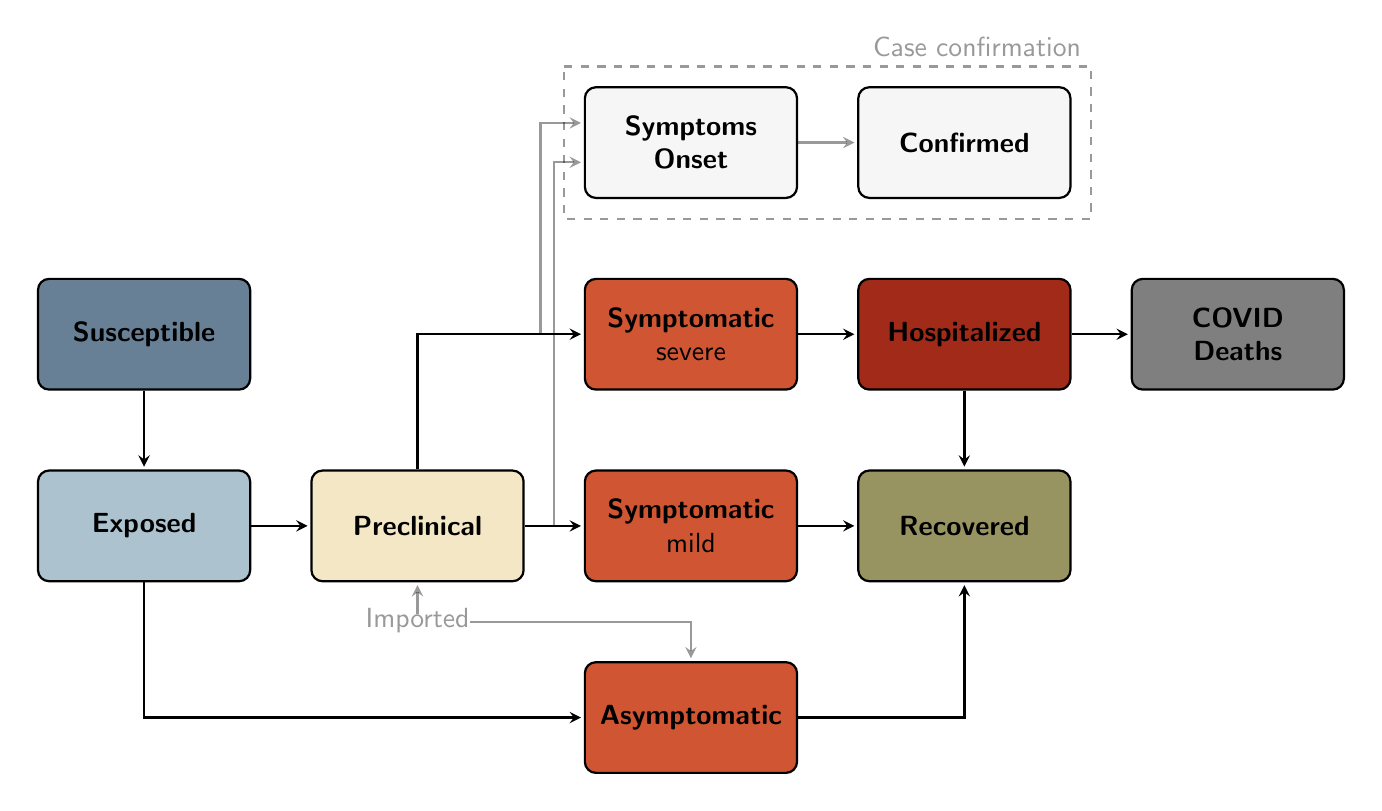
\begin{tikzpicture}[auto]
    \tikzstyle{hblock} = [rectangle, draw=black, thick, fill=susc, fill opacity=1,
    text width=7em, text centered, text opacity=1, rounded corners, minimum height=4em];
    \tikzstyle{preblock} = [rectangle, draw=black, thick, fill=pre, fill opacity=1,
    text width=7em, text centered, text opacity=1, rounded corners, minimum height=4em];
    \tikzstyle{iblock} = [rectangle, draw=black, thick, fill=inf, fill opacity=1,
    text width=7em, text centered, text opacity=1, rounded corners, minimum height=4em];
    \tikzstyle{cblock} = [rectangle, draw=black, thick, fill=care, fill opacity=1,
    text width=7em, text centered, text opacity=1, rounded corners, minimum height=4em];
    \tikzstyle{rblock} = [rectangle, draw=black, thick, fill=rec, fill opacity=1,
    text width=7em, text centered, text opacity=1, rounded corners, minimum height=4em];
    \tikzstyle{confblock} = [rectangle, draw=black, thick, fill=conf, fill opacity=1,
    text width=7em, text centered, text opacity=1, rounded corners, minimum height=4em];
    \tikzstyle{deadblock} = [rectangle, draw=black, thick, fill=dead, fill opacity=1,
    text width=7em, text centered, text opacity=1, rounded corners, minimum height=4em];
    \tikzstyle{expblock} = [rectangle, draw=black, thick, fill=exp, fill opacity=1,
    text width=7em, text centered, text opacity=1, rounded corners, minimum height=4em];
    \tikzstyle{line} = [draw, thick, -stealth,shorten >=1pt];
    \matrix (SIS) [column sep=0.75cm, row sep=1cm, ampersand replacement= \&]
      {
       % Row 1
       \& \& \node [confblock] (onset) {\textbf{Symptoms} \\ \textbf{Onset}}; \&
       \node [confblock] (confirmed) {\textbf{Confirmed}}; \\
       % Row 1 
       \node [hblock] (s0) {\textbf{Susceptible}}; \& \&
       \node [iblock] (symp1) {\textbf{Symptomatic} \\ severe}; \&
       \node [cblock] (hosp) {\textbf{Hospitalized}}; \&
       \node [deadblock] (deaths) {\textbf{COVID} \\ \textbf{Deaths}}; \\
       %Row 1
       \node [expblock] (exp) {\textbf{Exposed}}; \&
       \node [preblock] (pre1) {\textbf{Preclinical}}; \&
       \node [iblock] (symp2) {\textbf{Symptomatic} \\ mild}; \&
       \node [rblock] (rec) {\textbf{Recovered}}; \\ 
       %Row 2
       \& \& \node [iblock] (asymp) {\textbf{Asymptomatic}}; \\
      };

    \tikzstyle{every path}=[line]
      % % Drawing the links
      \draw (s0) -- (exp);
      \draw (exp) -- (pre1);
      \draw (pre1) |- (symp1);
      \draw (pre1) -- (symp2);
      \draw (exp) |- (asymp);
      \draw (symp1) -- (hosp);
      \draw (symp2) -- (rec);
      \draw (hosp) -- (rec);
      \draw (hosp) -- (deaths);
      \draw (asymp) -|  (rec);
      \draw [opacity=0.4] ([yshift=0.5cm, xshift=-2.8cm]asymp.north) -|  (asymp.north) ;
      \draw [opacity=0.4] ([yshift=-0.40cm]pre1.south) -- node[below, opacity=0.4]{Imported}  (pre1.south) ;
      \draw [opacity=0.4] ([xshift=0.375cm]pre1.east) -| ([xshift=-0.375cm,yshift=-0.25cm]onset.west) |- ([yshift=-0.25cm]onset.west); 
      \draw [opacity=0.4] ([xshift=0.2cm, yshift=2.45cm]pre1.east) -- ([xshift=-0.55cm,yshift=0.25cm]onset.west) |- ([yshift=0.25cm]onset.west); 
      \draw [opacity=0.4] (onset) -- (confirmed);
      \draw[opacity=0.4,-, dashed] ([xshift=-0.25cm, yshift=0.25cm]onset.north west) -| node[above left, opacity=0.4]{Case confirmation} ([xshift=0.25cm, yshift=-0.25cm]confirmed.south east) -| ([xshift=-0.25cm, yshift=0.25cm]onset.north west);
\end{tikzpicture}

\end{document}